\documentclass[12pt]{article}
\usepackage[dvips]{graphicx}
%\usepackage{epsfig}
\usepackage{verbatim}
\linespread{1.5}
\usepackage[margin=1in]{geometry}
% \addtolength{\textwidth}{3cm}
% \addtolength{\hoffset}{-2cm} \addtolength{\textheight}{3cm}
% \addtolength{\voffset}{-1.5cm}
\usepackage{rotating}
\usepackage{multirow}
\usepackage{subfig}
\usepackage{pdflscape}
\usepackage{amsmath,amstext,amsopn,amsxtra,amsgen,amsbsy,amscd,amssymb}
\usepackage{multirow}
\usepackage{setspace}
\usepackage{booktabs}
\usepackage{threeparttable}
\usepackage{wasysym}

% Bib
\usepackage[authoryear]{natbib}                           % Bibliography
% \makeatletter
% \def\@mb@citenamelist{cite,citep,citet,citealp,citealt,citeauthor} % allow citeauthor with multibib
% \makeatother
% \usepackage[resetlabels]{multibib}
\usepackage{url}                                          % Allows urls in bib
% \newcites{App}{Online Appendix References}
%% The new list's label is "App" and will be titled "Appendix References".
%% To put cites into this list, use \citeApp, \citetApp, \citepApp, ...
% \newcites{Add}{Addendum References}
%% The new list's label is "App" and will be titled "Appendix References".
%% To put cites into this list, use \citeApp, \citetApp, \citepApp, ...

\newtheorem{definition}{Definition}[section]
\newtheorem{theorem}{Theorem}
\newenvironment{proof}[1][Proof]{\begin{trivlist}
		\item[\hskip \labelsep {\bfseries #1}]}{\end{trivlist}}
\newenvironment{example}[1][Example]{\begin{trivlist}
		\item[\hskip \labelsep {\bfseries #1}]}{\end{trivlist}}
\newenvironment{remark}[1][Remark]{\begin{trivlist}
		\item[\hskip \labelsep {\bfseries #1}]}{\end{trivlist}}


\usepackage{color}
\usepackage[dvipsnames]{xcolor}
\definecolor{darkblue}    {RGB}{0.  ,0.  ,139.}
\usepackage[normalem]{ulem}

\usepackage[backref=page]{hyperref}
% \usepackage{hyperref}
\hypersetup{unicode=true,bookmarksnumbered=true,bookmarksopen=true,bookmarksopenlevel=3,
 breaklinks=true,pdfborder={0 0 0},colorlinks,citecolor=darkblue,filecolor=darkblue,linkcolor=darkblue,urlcolor=Maroon}
\usepackage[all]{hypcap}
\usepackage{breakurl}
% \usepackage{doi}

% allow for multiple footnotes with hyperref:
\let\oldFootnote\footnote
\newcommand\nextToken\relax
\renewcommand\footnote[1]{%
    \oldFootnote{#1}\futurelet\nextToken\isFootnote}
\newcommand\isFootnote{%
    \ifx\footnote\nextToken\textsuperscript{,}\fi}

\begin{document}

%========================================
% FIGURES AND TABLES
%========================================

% Figure: Obesity, caloric availability, and exercise
%\begin{landscape}
\begin{figure}[ht]
    \centering
    \caption{US Adult Obesity Rate, Caloric Availability and Exercise, 1970--2020} 
    \label{fig:obesity_calories_exercise}
    
    \subfloat[Obesity rate (\%)]{
    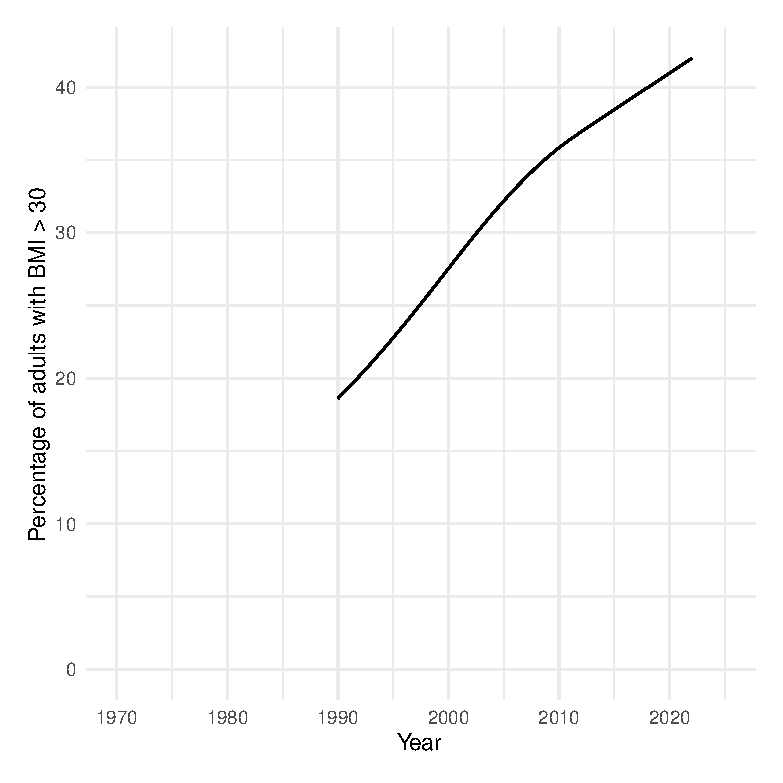
\includegraphics[width=0.45\textwidth]{../exhibits/figures/obesity-usa.eps}
    } \hfill
    \subfloat[Per-capita daily availability of calories (kcal)]{
    \includegraphics[width=0.45\textwidth]{../exhibits/figures/calories.eps}
    } \\
    \hfill \subfloat[Percentage of adults who meet the 2008 American physical activity guidelines for both aerobic and muscle-strengthening]{
    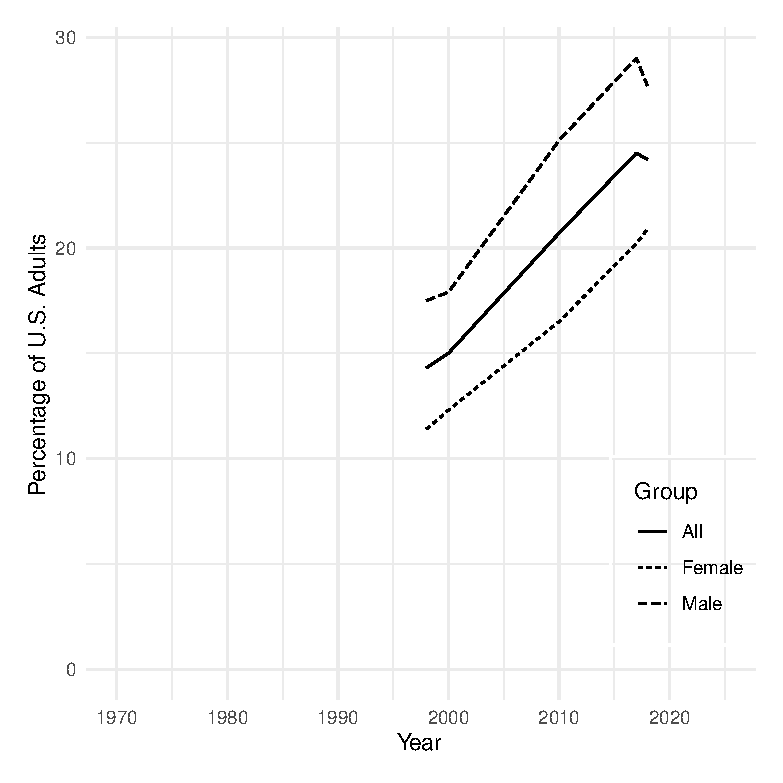
\includegraphics[width=0.45\textwidth]{../exhibits/figures/exercise.eps}
    } \hfill
    
    \begin{minipage}{\textwidth}
    \bigskip
    
    \footnotesize
    \textsc{Notes.}---Caloric availability is a measure of the total amount of food available for human consumption and is an estimate of total consumption. The USDA figure is adjusted for spoilage and waste.
    
    \bigskip
    \textsc{Sources.}---Obesity rate data from the World Health Organization's (WHO) Global Health Observatory (GHO). Caloric availability data from the USDA Economic Research Service or the United Nations Food and Agriculture Organization, accessed via the website ``Our World in Data.'' Data on physical exercise is taken from the National Center for Health Statistics' National Health Interview Survey, Family Core and Sample Adult questionnaires. 
    \end{minipage}
\end{figure}
%\end{landscape}

% Figure: Comparing food diary and agricultural sales data
\begin{figure}[ht]
    \centering
    \caption{Comparison of food diary and agricultural sales data, 2000--2022} 
    \label{fig:consump_compare}
    
    \subfloat[Average calories consumed per day (kcal)]{
    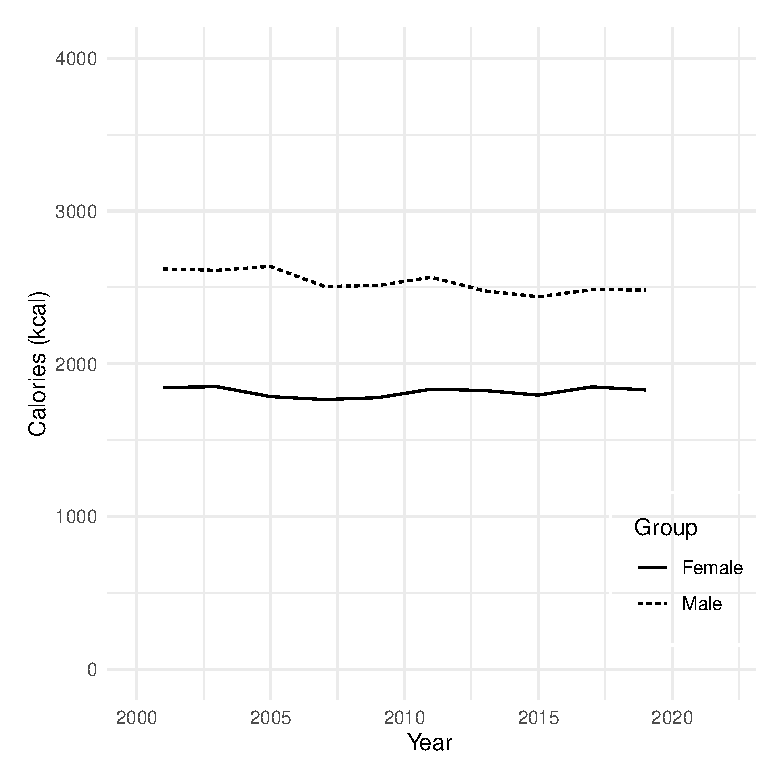
\includegraphics[width=0.33\textwidth]{../exhibits/figures/wweia_calories.eps}
    } \qquad
    \subfloat[Per-capita daily availability of calories (kcal)]{
    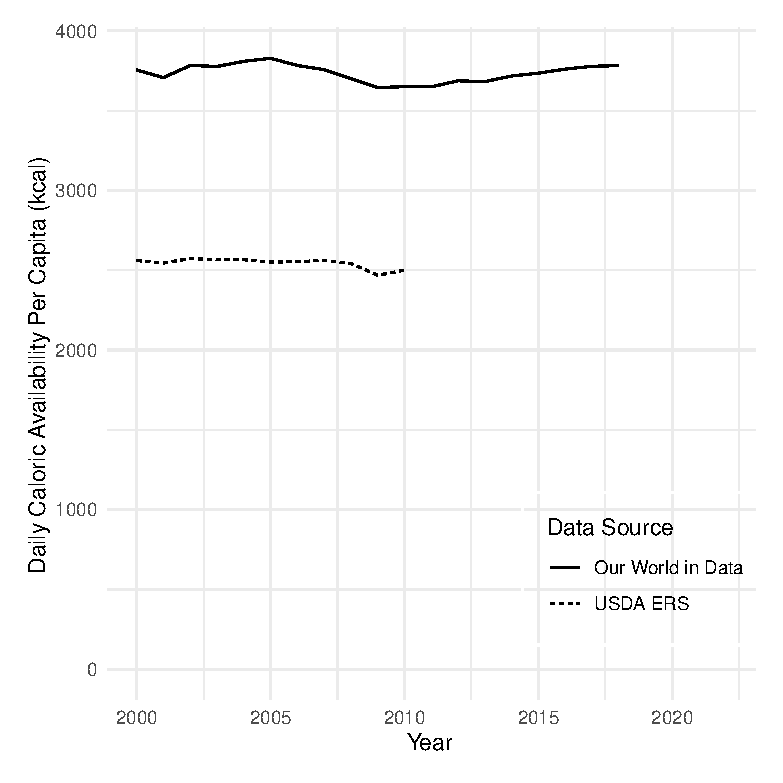
\includegraphics[width=0.33\textwidth]{../exhibits/figures/calories-since-2000.eps}
    } \\
    \subfloat[Average sugars consumed per day (g)]{
    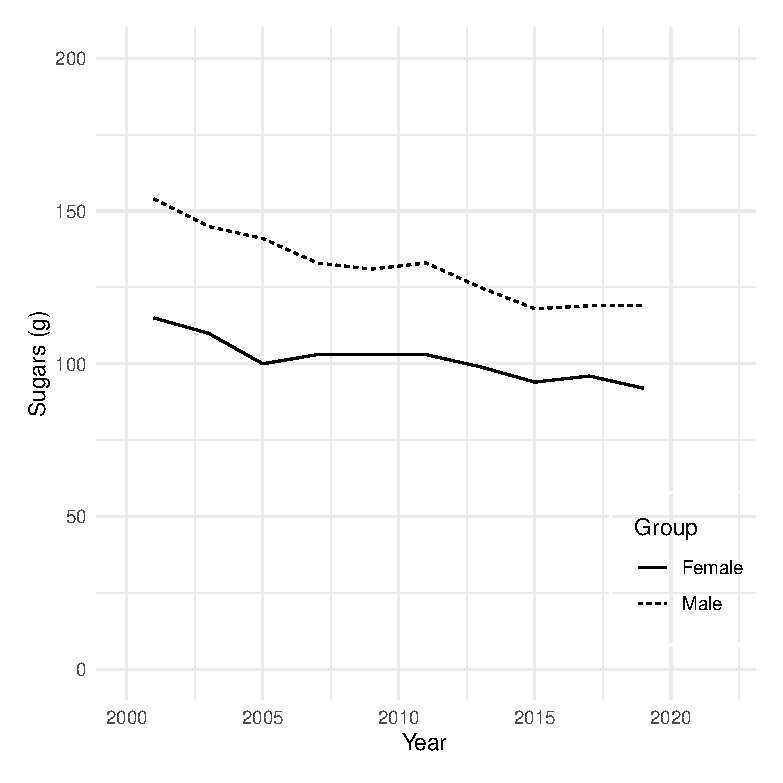
\includegraphics[width=0.33\textwidth]{../exhibits/figures/wweia_sugars.eps}
    } \qquad
    \subfloat[Per-capita daily availability of caloric sweeteners (g)]{
    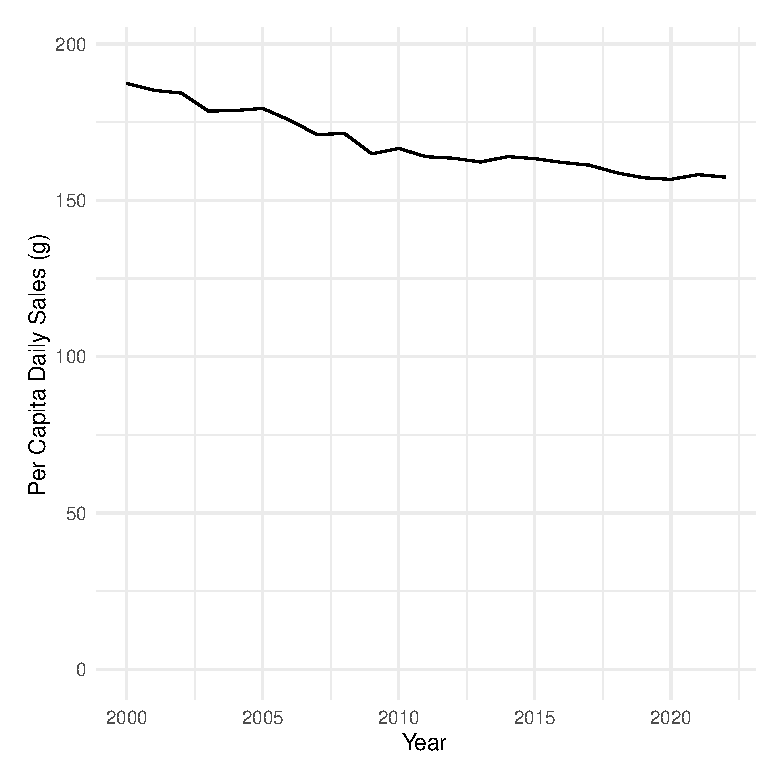
\includegraphics[width=0.33\textwidth]{../exhibits/figures/all-sweeteners-annual-since-2000.eps}
    } \\
    \subfloat[Average omega-6 PUFAs consumed per day (g)]{
    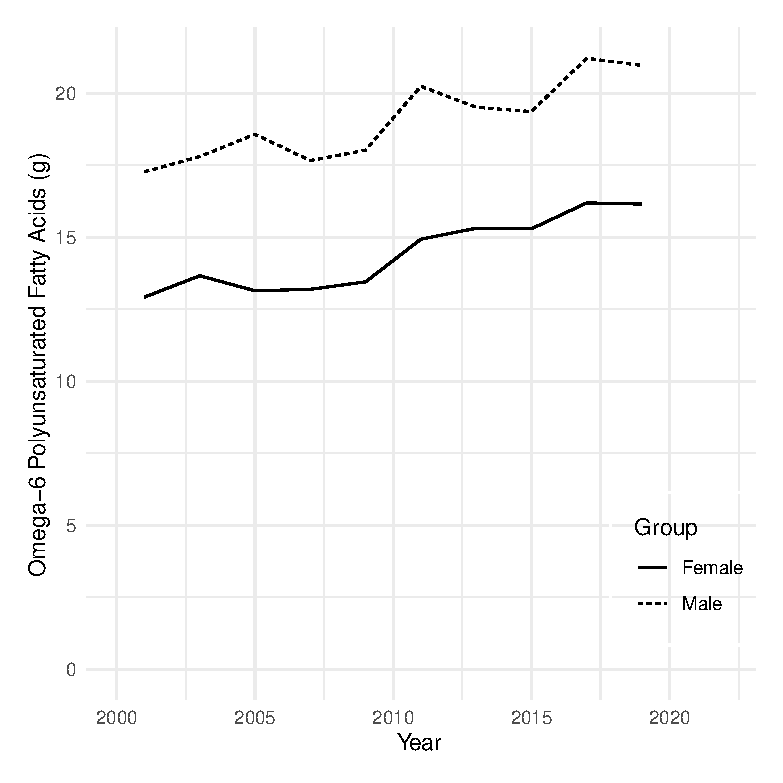
\includegraphics[width=0.33\textwidth]{../exhibits/figures/wweia_omega6.eps}
    } \qquad
    \subfloat[Per-capita daily disappearance of edible seed oils (g)]{
    \includegraphics[width=0.33\textwidth]{../exhibits/figures/all-seed-oils-annual-since-2000.eps}
    }
    
    \begin{minipage}{\textwidth}
    \bigskip
    
    \footnotesize
    \textsc{Notes.}---All quantities are converted to be in the same units and plotted on the same axes for ease of comparison. The lone exception is the seed oils graphs, as these scales were too far off to be comparable. One pound per annum is approximately equal to 1.24 grams per day.
    
    \bigskip
    \textsc{Sources.}---Consumption data comes from NHANES food surveys as aggregated by the USDA's ``What We Eat in America,'' respondents aged 20 and over. Agricultural sales data comes from the USDA Economic Research Service.
    \end{minipage}
\end{figure}


% Figure: Obesity and consumption of caloric sweeteners
\begin{figure}[ht]
    \centering
    \caption{US Adult Obesity Rate, Availability of Caloric Sweeteners, and Disappearance of Edible Seed Oils, 1970--2020} 
    \label{fig:obesity_sweeteners_seed_oils}
    
    \subfloat[Obesity rate (\%)]{
    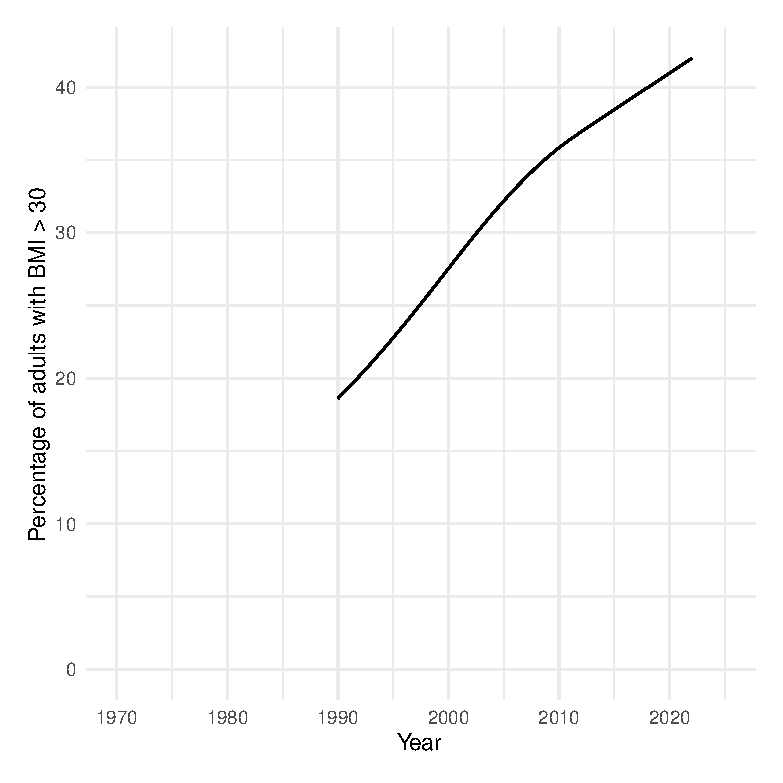
\includegraphics[width=0.45\textwidth]{../exhibits/figures/obesity-usa.eps}
    } \hfill
    \subfloat[Per-capita annual availability of caloric sweeteners (lbs.)]{
    \includegraphics[width=0.45\textwidth]{../exhibits/figures/all-sweeteners-annual.eps}
    } \\
    \hfill \subfloat[Per-capita annual disappearance of edible seed oils (lbs.)]{
    \includegraphics[width=0.45\textwidth]{../exhibits/figures/all-seed-oils-annual.eps}
    } \hfill
    
    \begin{minipage}{\textwidth}
    \bigskip
    
    \footnotesize
    \textsc{Notes.}---Caloric sweeteners include cane/beet sugar, high fructose corn syrup, and other sweeteners such as honey. Seed oils refer to canola, corn, cottonseed, palm kernel, palm, peanut, safflower, soybean, and sunflower oils. The disappearance of seed oils is a measure of the total amount of seed oils available for human consumption. The availability of both sets of commodities is an estimate of their total consumption.
    
    \bigskip
    \textsc{Sources.}---Obesity rate data from the World Health Organization's (WHO) Global Health Observatory (GHO). Data on caloric sweetener availability and edible seed oil disappearance comes from the USDA Economic Research Service.
    \end{minipage}
\end{figure}


\end{document}
